The overall architecture of the proposed integrated simulation framework is depicted in Figure \ref{fig:system_architecture}.
The proposed integrated simulation framework follows a layered design in which ns-3 remains the primary discrete-event simulator while Sionna RT is embedded as environment aware ray-tracing engine.
The main goal of the architecture is to preserve the mature protocol, traffic generation, scheduling capabilities of ns-3, Sionna RT handle ray-tracing which provide realistic site-specific propagation channel model, while leveraging GPU acceleration for computation intensive process

\begin{figure}[htbp]
    \centering
    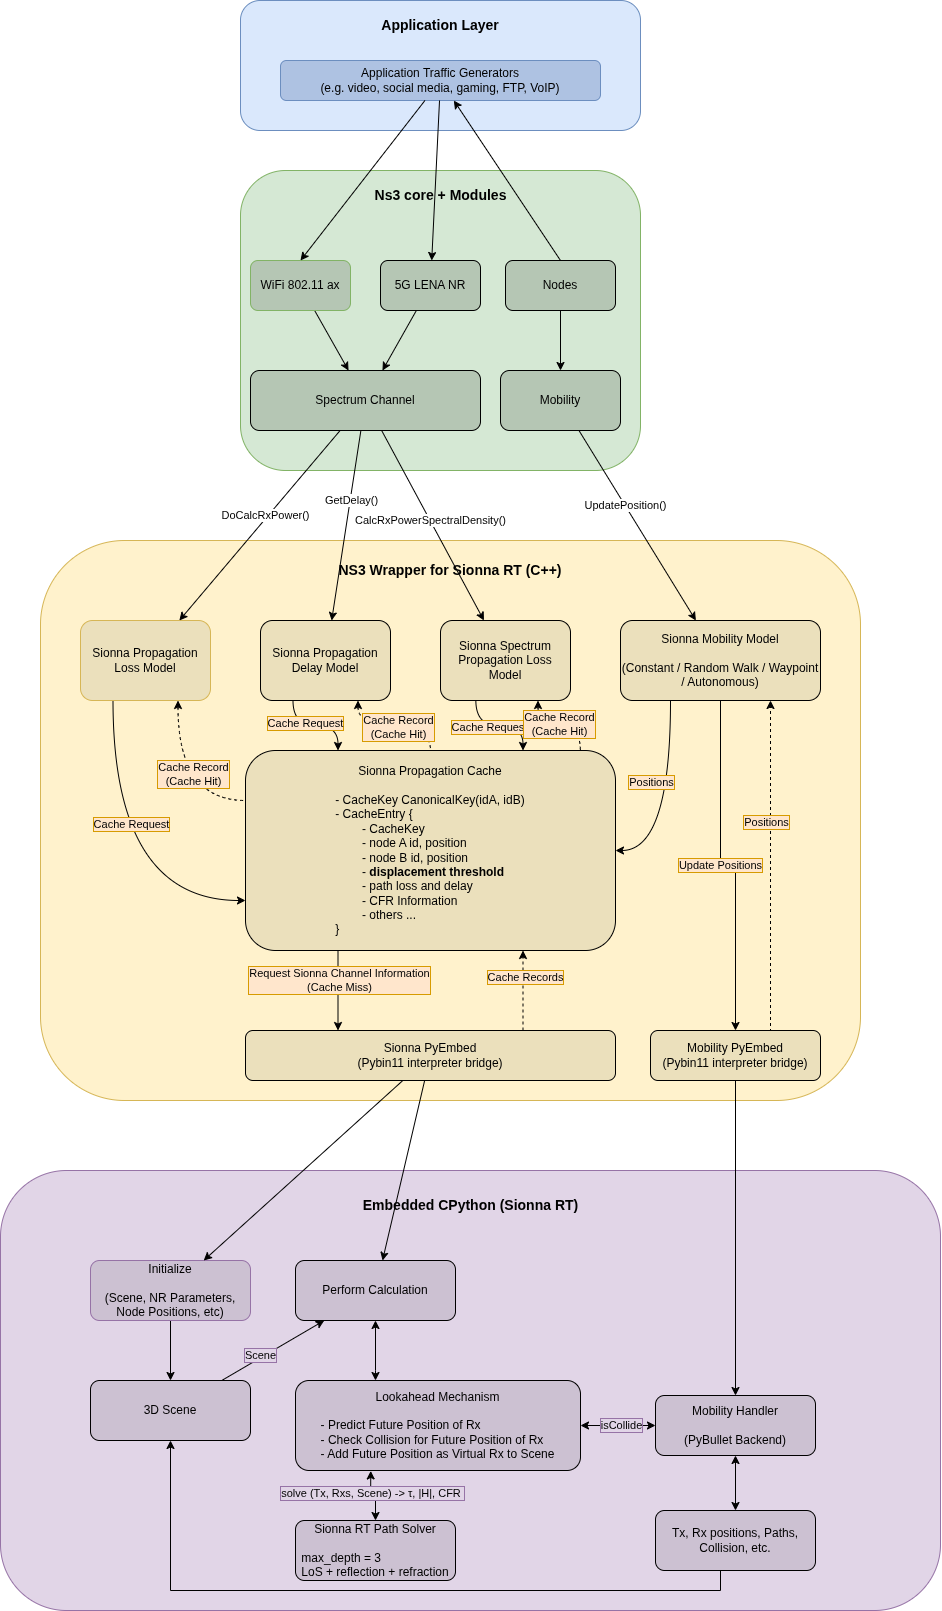
\includegraphics[width=\linewidth]{images/SionnaRT_System_Architecture.drawio.png}
    \caption{Architecture of the integrated simulation framework. }
    \label{fig:system_architecture}
\end{figure}

At the top is the application layer where the user defined traffic are generated between UEs and gNB.
These traffic can be of different type such as video streaming, social media, gaming, FTP and VoIP.
This traffic generators allow to simulate different workload scenarios which reflect the realistic network traffic behavior.

The middle layer colored in green is the network layer where the ns-3 stack is located.
Node manangement, mobility, routing, scheduling are handled by this layer.
It also handle MAC layer operation according to the chosen medium access and protocol standard.
For instance, the way packet processed for Wi-Fi 802.11ax or 5G NR is different and it is handled by the ns-3 MAC layer.
When a packet is generated by the application layer, it is first passed to the ns-3 stack.
Then, the ns-3 stack processes the packet according to the protocol stack.
Finally, the packet is transmitted over the wireless medium where it call \texttt{PropagationLossModel} and \texttt{PropagationDelayModel}, in order to calcualte path loss, transmission delay and channel fade.

When the call to \texttt{PropagationLossModel} and \texttt{PropagationDelayModel} triggered, the compuation of propagation delay and path loss is handled by the Sionna RT engine which provide environment aware channel information.
However, compuation these information using ray-tracing every time packet traverses is computationally intensive and it can significantly slow down the simulation.
To address this challenge, the next layer handle this issue using caching mechanism.
Whenever, a packet traverses between node A and node B, it check in cache for the channel information using their positions.
If the nodes are in positions where the calculated dispalcement distance is below the threshold value, it retrieve the channel information from cache as channel information relatively unchanged if they are under the coherence distance.
Otherwise, it trigger the ray-tracing engine to compute the channel information and update the cache with the new information.
In order to maximize the caching efficiency and reduce number to times it has to call the ray-tracing engine, future possible positions of the nodes are generated based on their current position and speed.

Then these generated positions are added to the scene as virtual receviers in additional to real receviers and the paths calculation is done by Sionna RT engine for all  receviers (real and virtual).
The channel information obtained for virtual receviers are added to the cahce for future use in addition to the channel information of the real positions.
This help to remove the need to call the ray-tracing engine every time packet traverses.
However, ns-3 can not directly call the Sionna RT engine to compute the channel information as they are written in different programming languages.
So, wrapper class is created to call Sionna RT engine from ns-3 in this layer.

Final bottom most layer which is in purple color is the Sionna RT engine where the ray-tracing is performed to compute the channel information.
Before the simulation starts, the radio propagation parameters, antenna configuration, and 3D scene information are initlized by passing the information form ns-3 side.
During the simulation, when the channel information requested is not in the cache, the calculation for future positions of the node, channel information for each node in different positions is calculated by using Sionna Path Solver.
Path solver calculate path loss, time of arrival, angle of arrival, angle of departure, etc based on the rays propagated in the 3D environment.
These calculation are done on GPU for efficient computation which give substantial performance.
Finally, the calculated channel information is returned to the ns-3 side through the wrapper class and updated in the cache.
